\documentclass{beamer}
\usetheme{metropolis}
\usepackage[utf8]{inputenc}
\usepackage{sansmathaccent} 
\pdfmapfile{+sansmathaccent.map}
\usepackage{mathtools}
\usepackage{amsmath}
\usepackage{amsfonts}
\usepackage{graphicx}
%\usefonttheme{serif}

%------------Serve per fare vedere le pallucelle e i numeretti nell'indice---------------%
\setbeamertemplate{section in toc}{%
	{\inserttocsectionnumber.}~\inserttocsection    \vspace{-.1\baselineskip}}
\setbeamercolor{subsection in toc}{bg=white,fg=structure}
\setbeamertemplate{subsection in toc}{%
	\hspace{0.2cm}{\begin{minipage}[c]{0.1em}\circle*{3}\end{minipage}}~\inserttocsubsection\par}
\setbeamerfont{subsection in toc}{size=\small}
%----------------------------------------------------------------------------------------%
\title[]{Secure Compression and Pattern Matching Based on Burrows-Wheeler Transform}
\institute{Università degli Studi di Salerno}
\author{Raffaele Ceruso Giovanni Leo}
\logo{
\includegraphics[scale=0.05]{Immagini/logoUnisa.png}}
\date{\today}

\AtBeginSection[]
{
	\begin{frame}
	\frametitle{Outline}
	\tableofcontents[currentsection] 
	\end{frame}
}
\begin{document}
\begin{frame}
\titlepage
\end{frame}
\begin{frame}
	\frametitle{Outline}
	\tableofcontents
\end{frame}
\section{Idea}
\begin{frame}
\frametitle{Idea}
	\begin{itemize}
		\item Le ``compressed data structure'' permettono di creare una indicizzazione di grandi dataset in maniera efficiente. Tali strutture dati dovranno essere sicuramente memorizzate in qualche server di terze parti come ad esempio il cloud, questo però porta sicuramente problemi di privacy. \pause
		\item L’ idea quindi é quella di costruire una variante di tali strutture più sicura, basata sulla trasformata di Burrows-Wheeler, e che sia in grado anche di eseguire il pattern matching.
	\end{itemize}
\end{frame}
\section{Introduzione}
\begin{frame}
\frametitle{Introduzione - 1}
	\begin{itemize}
	 \item La compressione dati non solo riduce lo spazio occupato dai file ma serve anche a migliorare la velocità di trasmissione in alcuni protocolli.
	 \pause
	 \item Essendo in era in cui i dati sono diventati veramente importanti di conseguenza anche la compressione di tali dati è diventata sempre più necessaria.
	 \pause
	 \item Gli autori del paper si sono focalizzati sull’utilizzo di algoritmi di compressione, i quali non solo supportano una compressione di tipo lossless ma che garantiscono anche sicurezza.
	 \pause
	 \item Il pattern matching è una operazione fondamentale nel processing delle stringhe che permette di trovare tutte le occorrenze di un dato pattern in un dato testo.
	 \end{itemize}
\end{frame}

\begin{frame}
\frametitle{Introduzione - 2}
	\begin{itemize}
		\item Il pattern matching si vuole applicare anche ai file compressi
		\pause
		\item Una possibile strategia potrebbe essere quella di decomprimere il file e cercare sul file decompresso ma tale strategia è poco efficiente.
		\pause
		\item Un approccio migliore sarebbe quello di ricercare direttamente sul file compresso \pause
		\item Per fare ciò abbiamo bisogno di indici di dati compressi i quali vengono salvati in server di terze parti causando problemi di privacy. 
		\pause
		\item Una semplice soluzione potrebbe essere quella di di comprimere e poi cifrare i dati ma tale soluzione è stata dimostrata non tanto sicura.
		\pause
		\item Una altra soluzione potrebbe essere quella di integrare compressione e cifratura in un unico passo ma anche questa soluzione presenta problemi di sicurezza.
		
	\end{itemize}
\end{frame}

\begin{frame}
\frametitle{Introduzione - 3}
	\begin{itemize}
		\item La soluzione proposta dagli autori si basa sulla trasformata di Burrows-Wheeler. Oltre la compressione tale trasformata può essere utilizzata anche per eseguire la ricerca. Se consideriamo due tabelle che forniscono un certo tipo di informazioni come per esempio la frequenza dei simboli e le posizioni, la trasformata permette di estrarre le sottostringhe che matchano i pattern in modo semplice.
		\pause
		\item Gli autori in questo paper forniscono un ``secure compression algorithm'' e un “secure compressed pattern matching”, entrambi basata sulla BWT. Inoltre viene uno schema di cifratura omomorfico additivo per proteggere gli indici dei dati compressi e per sfruttare le potenzialità del cloud. Per ottenere i dati dal server viene utilizzato il ``Private Information Retrival Read''(PIR\_Read).
		
	\end{itemize}
\end{frame}
\note[itemize]{
	\item La crittografia omomorfica è una forma di crittografia che consente il calcolo su testi cifrati(In questo caso la somma), generando un risultato crittografato che, decodificato, corrisponde al risultato delle operazioni come se fossero state eseguite sul testo in chiaro.\pause
	\item PIR\_Read: un modo privato per ottenere dati dal server
}
\section{Preliminari}
\subsection{BWT and compression}
\begin{frame}
\frametitle{Preliminari - 1 - BWT and compression}
	\begin{itemize}
	 \item BWT riorganizza una stringa di caratteri in una serie di caratteri simili quindi la si può vedere come un algoritmo che prepara i dati per usarli con delle tecniche di compressione dati.\pause
	 \item Adesso consideriamo una tale trasformazione in maniera generale divisa in tre passi:\pause
	 \begin{enumerate}
	 	\item Aggiungiamo un carattere speciale \$, il quale non è nell'alfabeto $\Sigma$, alla fine della stringa \textit{T} e assumiamo che \$ è il più piccolo carattere in $\Sigma$ considerando un ordine lessicografico.\pause
	 	\item Costruiamo una matrice \textit{M} le quali righe sono degli shift ciclici di \textit{T}.\pause
	 	\item Ordiniamo le righe della matrice \textit{M} in ordine lessicografico e diamo come output l’ultima colonna della matrice \textit{M}, il quale è il risultato della BWT.	\pause
	 \end{enumerate}
	\end{itemize}
\end{frame}

\begin{frame}
\frametitle{Preliminari - 1 - BWT and compression (Esempio BWT)}
 \begin{figure}[H]
 	\centering
 	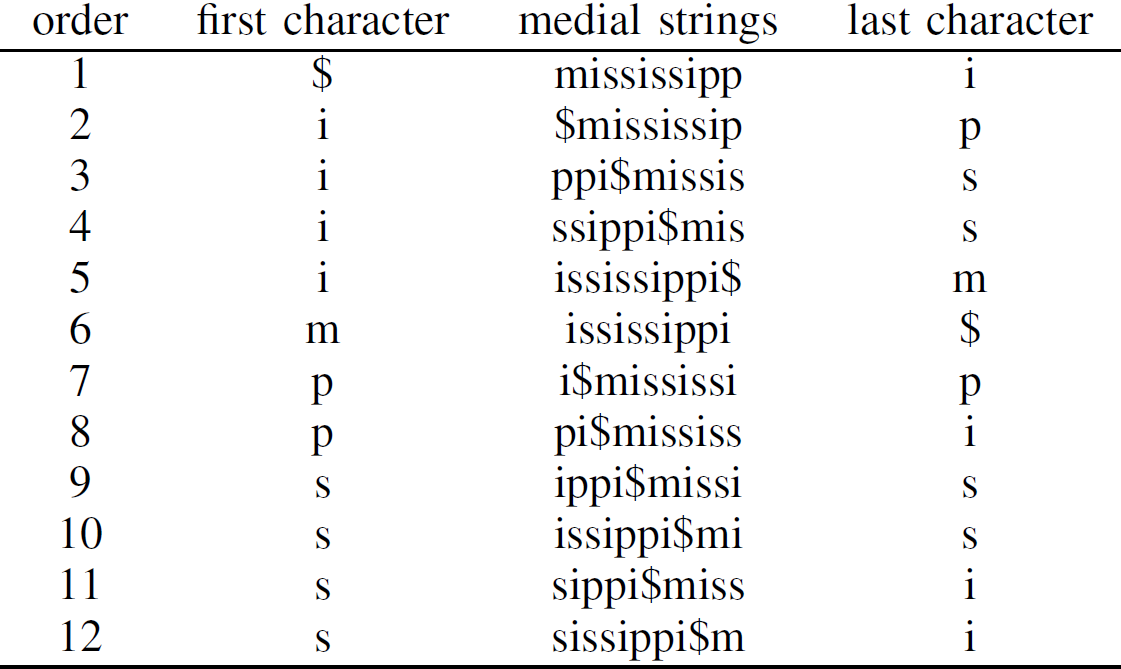
\includegraphics[scale=0.45]{Immagini/BWTExample}
 	\caption{Consideriamo l'esempio per la stringa ``mississippi\$''}
 \end{figure}
\end{frame}

\begin{frame}
 \frametitle{Preliminari - 1 - BWT and compression}
 \begin{itemize}
 	\item BWT è solo il primo passo di un algoritmo di compressione, di solito i passi sono: \textit{BWT+MTF+RLE+PC.}\pause
 	\item In maniera generale possiamo dire che la BWT cerca di raccogliere gli stessi caratteri insieme; MTF vuole rimpiazzare questi caratteri successivi uguali con degli zero; RLE vuole codificare questi zero con meno bit e infine PC vuole codificare il risultato della fase precedente in forma binaria. 
 \end{itemize}
\end{frame}

\begin{frame}
\frametitle{Preliminari - 1 - BWT and compression}
	\begin{itemize}
		\item BWT è solo il primo passo di un algoritmo di compressione, di solito i passi sono: \textit{BWT+\textbf{MTF}+RLE+PC.}\pause
		\item \textbf{MTF}(Move to front): Sia T il risultato della BWT, \textit{T=BWT(T)}. C'è una \textit{MTF\_table} contenente tutti i caratteri dell'alfabeto. La tabella mappa i caratteri alla loro relativa posizione nella tabella(per esempio il primo carattere è mappato a ``0''). Dopo aver codificato il primo carattere esso verrà spostato in prima posizione nella \textit{MTF\_Table} quindi tale carattere verrà mappato a ``0''. Sia \textit{Z =MTF(T)} ovvero la stringa codificata dopo aver applicato la MTF a \textit{T}.
	\end{itemize}
\end{frame}

\begin{frame}
\frametitle{Preliminari - 1 - BWT and compression}
\begin{itemize}
	\item BWT è solo il primo passo di un algoritmo di compressione, di solito i passi sono: \textit{BWT+\textbf{MTF}+RLE+PC.}\pause
	\item \textbf{Esempio MTF:}
	\begin{figure}[H]
		\centering
		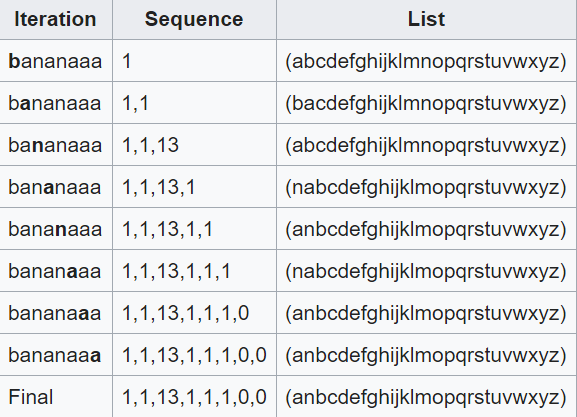
\includegraphics[scale=0.5]{Immagini/MTFExample}
	\end{figure}
	
\end{itemize}
\end{frame}

\begin{frame}
\frametitle{Preliminari - 1 - BWT and compression}
\begin{itemize}
	\item BWT è solo il primo passo di un algoritmo di compressione, di solito i passi sono: \textit{BWT+MTF+\textbf{RLE}+PC.}\pause
	\item \textbf{RLE}(Run Length Encoding): Possiamo applicare RLE per ogni run(sequenza di caratteri tutti uguali) di zero in $ Z $. Per essere più precisi possiamo rimpiazzare $ m $ successivi zeri con il valore binario del numero \textit{(m+1)}, scartando il bit più significativo, in ordine inverso. Inoltre introduciamo altri due caratteri\textit{ \textbf{a}} e \textit{\textbf{b}}  per fare la codifica degli zero. Per esempio 5 zeri vengono codificati come ab. Inoltre il risultato è su di un alfabeto \{\textbf{\textit{a}},\textbf{\textit{b}},1,...,$|\Sigma-1|$\}  dove $|\Sigma|$ indica il numero di caratteri presenti nell'alfabeto.
\end{itemize}
\end{frame}

\begin{frame}
\frametitle{Preliminari - 1 - BWT and compression}
\begin{itemize}
	\item BWT è solo il primo passo di un algoritmo di compressione, di solito i passi sono: \textit{BWT+MTF+RLE+\textbf{PC}.}\pause
	\item \textbf{PC}(Variable Length prefix code): Possiamo applicare Variable Length prefix code a questi simboli dell'alfabeto $ \{a,b,1,...,|\Sigma| -1\} $. Codifichiamo \textbf{a}  con 10 e \textbf{b}  con 11. Per gli altri simboli i usiamo $ 1+2* \lfloor log(i+1) \rfloor $  dove  $\lfloor log(i+1) \rfloor$   bit  sono 0 seguiti dal numero (i+1)  nella forma binaria costituita da 1 +  $\lfloor log(i+1) \rfloor$   bit, per esempio 00110 per il simbolo ``5''. Quindi il risultato finale è sull’alfabeto \{0,1\} e denotiamo il risultato finale \textit{BZ = PC(RLE(Z))}.
	
\end{itemize}
\end{frame}

\subsection{Strutture dati ausiliarie e backward pattern matching}

\begin{frame}
\frametitle{Preliminari - 2 - Strutture dati ausiliarie e backward pattern matching}
\begin{itemize}
	\item Per supportare il backward pattern matching abbiamo bisogno di due strutture dati ausiliarie:\pause
	\begin{enumerate}
		\item \textbf{c(e)}:la quale è una tabella che memorizza l'indice minimo di una stringa che inizia con il carattere \textit{e} nella matrice ordinata \textit{M} e denotiamo il prossimo simbolo il quale è un po più grande del simbolo e  in ordine lessicografico, con \textit{e+1}. Quindi \textit{c[e+1]- 1} restituisce la posizione finale di \textit{e}.\pause
		\item \textbf{occ(e,h)}: la quale memorizza le occorrenze di un carattere \textit{e} dalla prima fino ad una certa posizione \textit{h} nel risultato della BWT. 
	\end{enumerate}
\end{itemize}
\end{frame}

\begin{frame}
\frametitle{Preliminari - 2 - Strutture dati ausiliarie e backward pattern matching}

	\begin{itemize}
		\item \textbf{Lemma 1}: Data una stringa $ T_{1}=t_{1}...t_{n-1}t_{n}$  la quale è la h-esima stringa nella matrice ordinata M, sia $ T_{2} = t_{n}t_{1}...t_{n-1} $ la k-esima stringa nella matrice ordinata M, dove $ k = c[t_{n}] + occ(t_{n},h-1). $\pause
		\item La correttezza di tale lemma é data dal fatto che la matrice M é ordinata
	\end{itemize}
\end{frame}
\begin{frame}
\frametitle{Preliminari - 2 - Strutture dati ausiliarie e backward pattern matching}

\begin{itemize}
	\item Supponiamo di conoscere la stringa  ``sissippi\$mis'' che si trova nella posizione 10 e vogliamo sapere la posizione della stringa ``ssissippi\$mi'' quindi si ha che \\ \textit{c(s) + occ(s,9) = 9+3 = 12} e quindi sapremo che  ``ssissippi\$mi'' si trova in posizione 12.
\end{itemize}
\begin{figure}
	\centering
	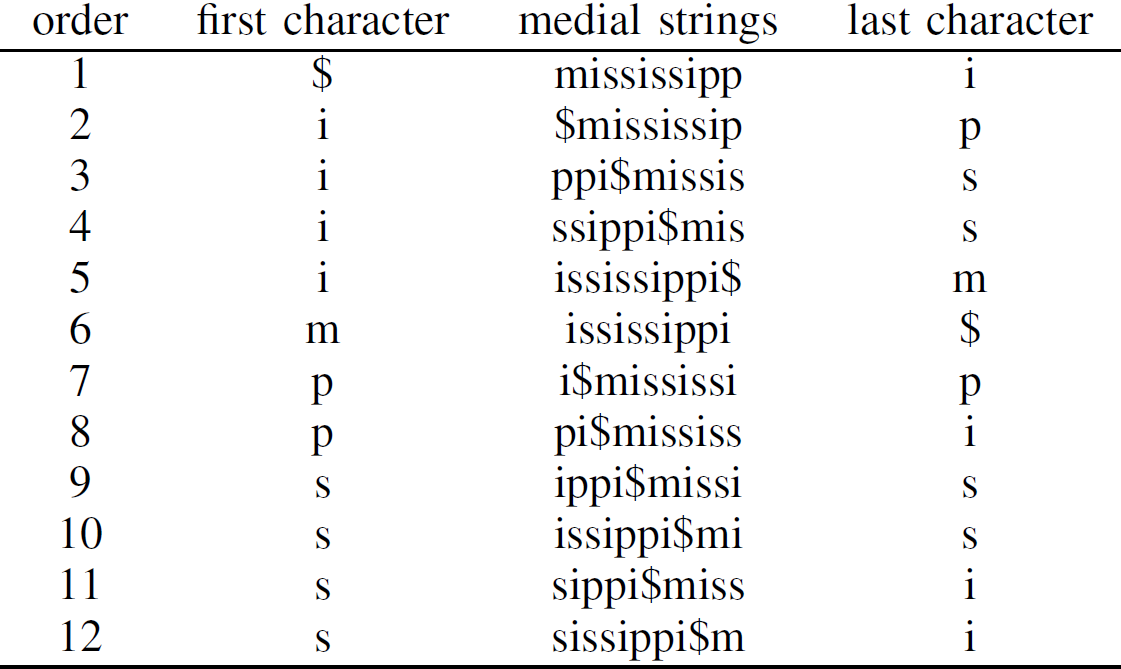
\includegraphics[scale=0.3]{Immagini/BWTExample.PNG}
\end{figure}
\end{frame}

\begin{frame}
\frametitle{Preliminari - 2 - Strutture dati ausiliarie e backward pattern matching - 1}
	\begin{itemize}
		\item \textbf{Lemma 2}:  Dato un pattern  $ P = p_{1}...p_{n} $  e un range (begin,end) nella matrice M dove queste stringhe iniziano con un subpattern $ p_{i+1}...p_{n} $ $ (i \geq  1) $, allora il range di $ p_{i}...p_{n} $ è \textit{(begin',end')}, dove $ begin' = c[p_{i}]+occ[p_{i},begin-1] $ e $ end' = c[p_{i}]+occ[p_{i},end] -1 $\pause
		\item Il risultato T della BWT può essere suddiviso in blocchi(block) di \textit{L} caratteri, inoltre \textit{L} blocchi vengono chiamati superblocchi(superblock). \textit{superblock(e,h)} restituisce l'occorrenza del simbolo e nei primi $ \lfloor h/L^{2} \rfloor $ superblocchi. \textit{block(e,h)} restituisce le occorrenza di e a partire dall’ultimo blocco fino al  $ \lfloor h/L \rfloor $ - esimo blocco. 
	\end{itemize}
\end{frame}

\begin{frame}
\frametitle{Preliminari - 2 - Strutture dati ausiliarie e backward pattern matching - 2}
	\begin{itemize}
		\item Per l'occorrenza in un blocco viene memorizzata in $ block\_inner(mtf(i),BZ_{i},e,h-i*L) $, dove $ BZ_{i} $ è l’i-esimo blocco compresso e mtf(i) memorizza lo stato della tabella MTF all’inizio della codifica dell'i-esimo blocco.	
	\end{itemize}
\end{frame}

\section{Costruzione}
\subsection{Compressione}
\begin{frame}
\frametitle{Costruzione- 3 - Compressione}
	\begin{itemize}
		\item Hanno provato a proporre un algoritmo di compressione che andava a combinare la sBWT con una variante del MTF dove la MTF table veniva inizializzata con lo stesso ordine lessicografico della sBWT, ma questo ha portato a problemi di sicurezza e quindi tale approccio è stato abbandonato.\pause
		\item Per risolvere tale problema gli autori hanno cambiato, in maniera random, la MTF table per ogni L caratteri(ovvero ogni blocco). Per ridurre la archiviazione delle chiavi per la funzione pseudo casuale, viene utilizzato come input per tale funzione il valore hash dell'ultimo blocco compresso.
	\end{itemize}
\end{frame}

\begin{frame}
\frametitle{Costruzione- 3 - Compressione}
\begin{itemize}
	\item L’algoritmo può essere visto in maniera generale come \textit{Algo=sBWT+bMTF+RLE+PC.}\pause
	\item Un utente sceglie una funzione funzione hash \textit{f} e una pseudo casuale funzione di permutazione \textit{Perm} basata su chiave. Poi sceglie un numero random per la funzione di permutazione come chiave(\textit{key}) privata. Quindi quando viene inserita un stringa l’utente la processa prima attraverso la sBWT e poi attraverso la bMTF. 
\end{itemize}
\end{frame}

\begin{frame}
\frametitle{Costruzione- 3 - Compressione}
\begin{itemize}
	\item L’algoritmo può essere visto in maniera generale come \textit{Algo=\textbf{sBWT}+bMTF+RLE+PC.}\pause
	\item \textbf{sBWT}(Scrambling BWT): Sia T la stringa originale e T = sBWT(T) il risultato della Scrambling BWT su T\pause
		\begin{itemize}
			\item Scegliamo un numero random r e dopo calcoliamo$  Perm(key,r) \rightarrow \xi $, dove $ \xi $ denota l’ordine lessicografico segreto.\pause
			\item Aggiungiamo un carattere parziale $\$ \notin \Sigma$ alla fine di T e assumiamo che \$ è il più piccolo dei caratteri dell'alfabeto $\Sigma$ nell’ordine lessicografico segreto $\xi$. Per semplicità chiamiamo la nuova stringa ottenuta T.\pause
			\item Costruiamo una matrice  \textit{M} le cui righe sono degli shift ciclici di di \textit{T}.\pause
			\item Ordiniamo le righe della matrice M utilizzando l’ordine lessicografico segreto $\xi$  e l’ultima colonna di \textit{M} è \textit{T}
		\end{itemize}
\end{itemize}
\end{frame}

\begin{frame}
\frametitle{Costruzione- 3 - Compressione - bMTF - 1}
	\begin{itemize}
		\item L’algoritmo può essere visto in maniera generale come Algo=sBWT+\textbf{bMTF}+RLE+PC\pause
		\item \textbf{bMTF}(blocky MTF): Raggruppiamo \textit{T} in blocchi di \textit{L} caratteri. Per ogni blocco scegliamo una permutazione dell’alfabeto prima a caso e dopo seguendo i passi della MTF per fare la codifica di qualsiasi carattere presente in ogni blocco. Qui verrà chiamata la funzione di permutazione pseudocasuale \textit{Perm} con due parametri la chiave e un nounce. Il nounce è un vettore \textit{IV} per il primo blocco ed è il valore hash dell’ultimo blocco codificato in altri casi.
		
	\end{itemize}
\end{frame}


\begin{frame}
\frametitle{Costruzione- 3 - Compressione - bMTF - 2}
	\begin{itemize}
	\item Procedimento schematizzato\pause
		\begin{itemize}
			\item Costruisci blocchi di \textit{L} caratteri a partire dalla stringa \textit{T}\pause
			\item Per il blocco i vine prima generata una\\ MTF\_table:$ Perm(key,IV$ or $f(block_{(i-1)}))\rightarrow bMTF\_table_{i} $, dove $ bMTF\_table_{i} $ è una permutazione di tutti i caratteri dell'alfabeto.\pause
			\item Segui gli step generali della MTF\pause
		\end{itemize}	 
	\end{itemize}
\end{frame}
\begin{frame}
\frametitle{Costruzione- 3 - Compressione - bMTF - 2}
\begin{itemize}
	\item Procedimento schematizzato\pause
	\begin{itemize}
		\item Costruisci blocchi di \textit{L} caratteri a partire dalla stringa \textit{T}\pause
		\item Per il blocco i vine prima generata una\\ MTF\_table:$ Perm(key,IV$ or $f(block_{(i-1)}))\rightarrow bMTF\_table_{i} $, dove $ bMTF\_table_{i} $ è una permutazione di tutti i caratteri dell'alfabeto.\pause
		\item Segui gli step generali della MTF\pause
	\end{itemize}	 
\end{itemize}
\end{frame}
\begin{frame}
\frametitle{Costruzione- 3 - Compressione }
	\begin{itemize}
		\item L’algoritmo può essere visto in maniera generale come Algo=sBWT+bMTF+\textbf{RLE}+\textbf{PC}\pause
		\item I passi \textbf{RLE} e \textbf{PC} devono semplicemente andare a codificare utilizzando meno bit possibili. \pause
	\end{itemize}
\end{frame}
\subsection{Pattern Matching}
\begin{frame}
\frametitle{Costruzione- 3 - Pattern Matching - 1}
\begin{itemize}
	\item Utilizzando strutture dati ausiliarie si ha la perdita di informazioni riguardanti frequenza e ordine lessicografico il che è un problema per la sicurezza.\pause
	\item Per risolvere tale problema gli autori hanno pensato di cifrare tali strutture e di proporre un protocollo per eseguire il pattern matching. In maniera sintetica servono tre passi:\pause
	\begin{enumerate}
		\item Permutare la occ table al fine di nascondere le informazioni
		\item Adottare un metodi di ottenimento delle informazioni privato al fine di ottenere le entità dalla \textit{occ} table al fine di ottenere un risultato conforme.\pause
		\item Falsificare alcune richieste al fine di nascondere dati come \textit{begin} e \textit{end}\pause
		
	\end{enumerate}	 
\end{itemize}
\end{frame}
%-----------------------Inizio Parte di Raffaele--------------------------------%
\section{Protocollo}
\begin{frame}
\frametitle{Protocollo}
Il protocollo prevede le seguenti fasi:

\textbf{$(1)$ Inizializzazione.} Il client genera le strutture dati \textit{c} e \textit{occ}. \textit{occ} è generata nel seguente modo.

\begin{itemize}
	\item \textit{superblock}:
	
	scegli un primo $ p_{1} $ leggermente più grande
	di $n/L^{2}$, un numero diverso da zero $ \beta_{1} $ e scegli un generatore
	$g_{1}$ di $ Z^{*}_{p_{1}} $. Il client mantiene $ g_{1} \beta_{1} $ segreti. Per \textit{superblock} $ i $, memorizziamo quei dati nel $ (g^{i}_{1}\beta_{1})^{th} mod$ $p_{1}$
	(omettiamo $mod$ $ p_{1}$ nella parte restante) della tabella.
	Per le entries vuote inseriamo alcuni numeri casuali.
\end{itemize}
\end{frame}
\begin{frame}
\frametitle{Protocollo}
Il protocollo prevede le seguenti fasi:

\textbf{$(1)$ Inizializzazione.} Il client genera le strutture dati \textit{c} e \textit{occ}. \textit{occ} è generata nel seguente modo.

\begin{itemize}
\item \textit{block}:

scegli un primo $ p_{2} $ che è poco più grande di $n/L$,
un numero diverso da zero $ \beta_{2} $ e scegli un generatore $g_{2}$ di $ Z^{*}_{p_{2}} $.
Il client mantiene $ g_{2} \beta_{2} $ segreti. Per \textit{block} $ i $, memorizziamo quei dati nel $ (g^{i}_{2}\beta_{2})^{th} mod$ $p_{2}$
(omettiamo $mod$ $ p_{2}$ nella parte restante) della tabella.
Per le entries vuote inseriamo alcuni numeri casuali.
\end{itemize}
\end{frame}
\begin{frame}
\frametitle{Protocollo}
Il protocollo prevede le seguenti fasi:

\textbf{$(1)$ Inizializzazione.} Il client genera le strutture dati \textit{c} e \textit{occ}. \textit{occ} è generata nel seguente modo.

\begin{itemize}
\item \textit{Hash\_value}:

Memorizziamo il valore hash di $ (i-1)^{th} $ block
per il blocco $ i^{th} $. Il valore hash di $ (i-1)^{th} $ block
è memorizzato nella $ (g^{i}_{2}\beta_{2})^{th}$ entry della tabella $Hash_value$ .
Per le entries vuote inseriamo alcuni numeri casuali.
\end{itemize}
\end{frame}
\begin{frame}
\frametitle{Protocollo}
Il protocollo prevede le seguenti fasi:

\textbf{$(1)$ Inizializzazione.} Il client genera le strutture dati \textit{c} e \textit{occ}. \textit{occ} è generata nel seguente modo.

\begin{itemize}
\item \textit{Block\_inner}:


La riga \textit{Block\_inner}($mtf[i],BZ_{i}, e, h-L*i$) viene spostato su \textit{Block\_inner}\textit{(Hash\_value}[$g^{i}_{2}\beta_{2}], BZ_{g^{i}{\beta_{2}}}, e, \tau(key, h-L*i))$
dove $i = \lfloor h/L\rfloor$ e $\tau$ : $Z_{L} $ $\rightarrow$ $Z_{L} $ è una funzione di permutazione casuale.
\end{itemize}
\end{frame}
\begin{frame}
\frametitle{Protocollo}
Il protocollo prevede le seguenti fasi:

\textbf{$(1)$ Inizializzazione.}
Per calcolare $occ(e, h)$, il client deve inviare un vettore di posizione $pv(h) = (g_{1}^{h/L^{2}} \beta_{1}, g_{2}^{h/L} \beta_{2}, \tau(key, h-[h/L] * L) )$ al server.\\ 

Pertanto l'algoritmo è Algo = sBWT + bMTF + RLE + PC +P dove P è la permutazione. Dopo aver criptato i dati in $occ$ con AHE il client li invia al server il quale mantiene $c$. Successivamente sceglie un numero adeguato R come round di comunicazione.
\end{frame}

\begin{frame}
\frametitle{Protocollo}
Il protocollo prevede le seguenti fasi:\\
\textbf{$(2)$ Client:} invia un vettore posizione $pos$ e legge il vettore $V$ in accordo di $P[i-1]$
\end{frame}

\begin{frame}
\frametitle{Protocollo}
Il protocollo prevede le seguenti fasi:\\
\textbf{$(3)$ Server:} per ogni carattere dell'alfabeto e del $y^{th}$ vettore in $pos$, computa $B_{y}[\zeta]$ e ritorna ${a_{y}}_{y\in[1,4]}$
\end{frame}

\begin{frame}
\frametitle{Protocollo}
Il protocollo prevede le seguenti fasi:\\
\textbf{$(4)$ Client:} trova l'aspettato $a_{i1}$, $a_{i2}$ $\in {a_{y}}_{y\in[1,4]} $ e computa
\begin{itemize}
\item $occ(P[i-1], begin-1)$
\item $occ(P[i-1], end)$
\item $begin$
\item $end$
\\	Se $begin \leq end$ e $i \geq 2 $ vai allo step 2, altrimenti invia $pos$ al server. Se il round di comunicazione è $R$ vai al prossimo step.
\end{itemize}
\end{frame}

\begin{frame}
\frametitle{Protocollo}
\textbf{$(5)$ Client:} se $end < begin$ il pattern non è stato trovato, altrimenti l'occorrenza del pattern è $end - begin +1$
\end{frame}
%--------------------------------------------------------------------------%
\section{Analisi}
\begin{frame}
\frametitle{Analisi}
\begin{itemize}
	\item A causa della lunghezza delle stringhe, anche con differente entropia, si era notato che dopo la compressione tali stringhe erano distinguibili, nei modelli adottati in passato.\pause
	\item Gli autori hanno dimorato che  due stringhe isomorfe in ogni blocco dopo il passo della sBWT il risultato finale della compressione risulta indistinguibile.\pause
	\item Inoltre hanno dimostrato anche che il \textit{pattern matching} viene eseguito in un tempo accettabile ed è anche sicuro andando a fare particolari accorgimenti. 
\end{itemize}
\end{frame}

\note[itemize]{
	\item Stringhe della stessa lunghezza dove i caratteri della prima prima stringa possono essere rimpiazzati da quelli della seconda mantenendo l'ordine lessicografico
}
\begin{frame}
	\centering
	\large{Grazie per l'attenzione!}
\end{frame}
\end{document}